\chapter{Performance of  \migrate}
\myabstract{Markov chain Monte Carlo programs are difficult to use and despite what people tell you very error-prone. This chapter tries to convince you that \migrate often is doing the correct thing, and when something goes wrong that you perhaps can find out why and how it went wrong.}

Markov chain Monte Carlo samplers have the proven property that when they are run infinitely long they converge to the correct value, but since we cannot run the program infinitely long, we are interested how many samples we need to get before we start to get ``acurate" result.  This is true for maximum likelihood and Bayesian inference modes of the program.
Despite the huge literature about measures when to stop sampling, there
is still no good universal criteria available. \migrate reports some measures, such as the effective sample size of an MCMC run, or the Gelman-Rubin statistic. The problem of difficulty to converge can be divided into three simple categories: 
\begin{enumerate}
\item Programming errors, typically programs of this complexity will always contain some errors, programmers certainly try to make every effort to make sure that there are no errors in the main calculations, but testing is typically very difficult especially when interactions among multiple options, different hardware need to be tested. 
\item The sampler was not run long enough, this is data dependent and some general guidelines could be given, 
%NSF slant 1
but NSF panels do not seem too keen to fund projects that would do that. To my knowledge, no study has explored effects of sample size, sequence lengths/variability of sequence for more than a single population \citep{Pluzhnikov:1996, Felsenstein:2005, Carling:2007}. You have to explore this with your own data.
\item The assumptions of the model are not met, all data will violate some of the assumptions but typically the method is quite tolerant.
\end{enumerate}
I will discuss some ways to investigate these three sources of problems in the following paragraph, highlighting the potential source of error.

The program is sampling form the right distribution: 
running the sampler with no data (e.g. sequence data with all ``?'' data)
should result
in the distribution $\prob(G|\P_0)\prob(D|G)$, the one 
we sample from [checks {\bf (1)}]. With Bayesian inference the uninformative data runs will return the prior distribution [checks {\bf (1)}]. 

Large simulation studies show that we can recover parameters and 
population structure that was used to create the data
[checks {\bf (1,2)}].  Such simulations need to be planned very carefully because silly parameter combination may suggest that the method does not work, but we perhaps would hope that under biological useful parameter ranges the program should deliver good results, an example of a study where the parameter range was not optimal is a paper by \cite{Abdo:2004:EPL}. Real data may have difficulties to deliver consistent results, the most common source of this problem seems that either the model is heavily violated (non-neutral loci, non-random mating, very high rate of recombination). For many data sets this seems not to be a problem, so.
%\begin{wrapfigure}{20}{9cm}
\begin{figure}[htbp]
\begin{center}
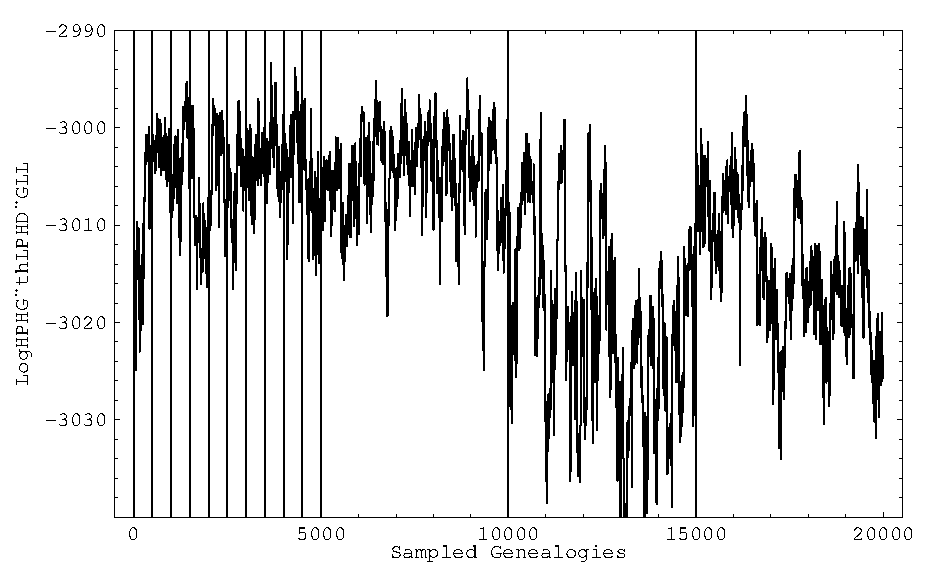
\includegraphics[width=12cm]{mim/mixing}
\end{center}
\vskip -0.5cm
\caption{Data likelihood $\prob(D|G)$ for all sampled genealogies: 
A sample run of migration estimation using 2 populations,
the very long vertical lines mark chain boundaries (10 short and
3 long chains). Totally, $10$ short chains $\times 500$ sampled genealogies 
$+ 3$ long chains $\times$ sampled $5000$ genealogies were sampled out of
total 400,000. The values for not recorded trees are 
not shown.
}
\label{FIGMIX}
\end{figure}
%\end{wrapfigure}

The program is sampling many different genealogies; one can show 
this by plotting
a curve showing on the x-axes all sampled trees and on the y-axis 
the likelihood of the genealogy (in our case this is $\prob(D|G)$
, Figure \ref{FIGMIX}). 
A plot of a sequence of $\prob(\P|G_i)\prob(D|G_i)$ is not 
useful because the genealogies contain different number of time intervals,
and they are {\bf not} comparable. 

One can show that starting from random start parameters, the estimates
converge rather quickly after a few short chains (Figure \ref{fig:convergence}), the updating of
the start parameters over several short chains moves the estimates to the
proper region and the remaining uncertainty is only driven by the
often huge uncertainty about the parameter estimates in the data, 
the likelihood surface is flat for many parameter combinations and 
the data. [checks {\bf (2)}] 
%\begin{wrapfigure}{18}{9cm}
\begin{figure}[hpbt]
%\vskip -1cm 
\begin{center}
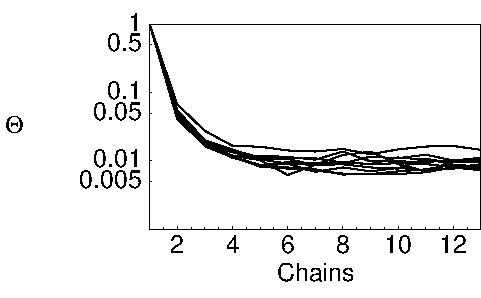
\includegraphics[width=12cm]{mim/convergence_singlepop}
\end{center}
\vskip -0.5cm
\caption{Convergence to the true parameter region. 
Ten runs were started from a $\Theta=1.0$. The data was generated using
a $\Theta=0.01$.
Totally, $10$ short chains $\times 500$ sampled genealogies 
$+ 3$ long chains $\times$ sampled $5000$ genealogies were sampled out of
total 400,000.
}
\label{fig:convergence}
\end{figure}
%\end{wrapfigure}

Comparison with other programs produce similar results. I compared
\migrate with \genetree \citep{Bahlo:2000:IGT} and with
{\tt fluctuate} \citep{Kuhner1998-429}. The comparison with \genetree
used two populations (England and Ghana: 2.5 kb sequence data for the 
beta-globin locus \citep{harding1997-772}) and the results were very similar.
For my paper on n-population I have worked out a 100-locus data set simulation
that shows that \genetree and \migrate deliver the same estimates, and
approximative confidence intervals, although
\genetree is very slow compared to \migrate  for that specific
data set \citep{beerli:2001:mle}.
\vskip 0.7cm 
The comparison with {\tt fluctuate} was for one population, yes you can run \migrate with only one population, and for a data set
created using a $\Theta=0.01$ \migrate delivered $\Theta=0.0123$
with a 50\% confidence interval of $0.08$ to $0.017$, 
while {\tt fluctuate} delivered a point estimate of $\Theta=0.0119$. 
\vskip 0.7cm
In 2007, \citeauthor{roychoudhury:2007:fae} published a new method to infer population-scaled mutation rates, their findings helped me to find a problem with my microsatellite estimator and now accuracy and speed are very similar to their estimator \citep[Figure \ref{fig:msatcomp}][]{beerli:2007:eps}. 
[checks {\bf (1,2)}] 
\vskip 0.7cm
\migrate Version 2.2 and newer print out statistics that help to assess whether the program was run long enough: (1) effective sample size [ESS] and (2) Rubin-Gelman statistic to assess convergence. I am not a strong believer of such measures because they only show the worst problems. For example effective sample sizes of 1000 may seem a lot but it certainly depends on the number of other parameters and the correlation among parameters. The program TRACER (Rambaut et al. 2005) flags effective sample sizes below 100; this is very low for population genetic purposes, I suggest that you strive to get at least 1000 or more for all parameters including the likelihood of the genealogies.
\vskip 1cm
\begin{figure}[hb]

\begin{center}
\includegraphics[width=12cm]{mim/biasfig_revised}

\end{center}
\caption{Mutation-scaled population size estimated from microsatellite data. Bias and absolute error for \migrate version 2.3. Left column: using the stepwise mutation model. Right column: using the Brownian motion approximation, Scale and calculations of bias and absolute error are the same as in Figure 1 in \cite{roychoudhury:2007:fae}. The open squares are the values for $\theta$=32 from their paper.
}
\label{fig:msatcomp}
\end{figure}
\clearpage
